%% Karlsruhe Institute of Technology
%% Institute for Anthropomatics and Robotics (IAR)
%% Artificial Intelligence for Language Technologies (AI4LT) lab
%%
%% Prof. Dr. Jan Niehues
%% Lab's website https://ai4lt.anthropomatik.kit.edu/english/index.php

\chapter{Evaluation}
\label{ch:Evaluation}
The evaluation of results of the experiments that were conducted on the benchmark section of the IWSLT 2023 dataset \cite{sperber2024evaluating} with regards to \ref{ch:Dataset} as the relevant changes and preprocessing that was done.

The resulting scores are then pearson correlated \cite{2020SciPy-NMeth} to comet scores as well as word error rates and compare those. 
\todo{maybe move evaluations metrics here?}
%% -------------------
%% | Example content |
%% -------------------


\section{Transcription evaluation}
To evaluate how good the transcription quality estimation is the Word error rate\footnote{the used WER implementation can be found here: https://github.com/analyticsinmotion/werpy} \ref{wer}, is used as reference score to compare the transcription quality estimation metric by correlating the WER scores with the help of the pearsoncorrelation \cite{2020SciPy-NMeth}
As WER is case sensitive, both the model result and the reference are normalised to be all lowercase, with single spaces, no leading or trailing blank spaces and no punctuation.
the resulting transcription probabilities plotted over the according WER values is shown in \ref{fig:transcript scatter plot} and the pearsoncorrelation can be found in \ref{transcription results}
\todo{add (scatter)plot with model and reference prob plotted, expand}
\begin{figure}
    \centering
    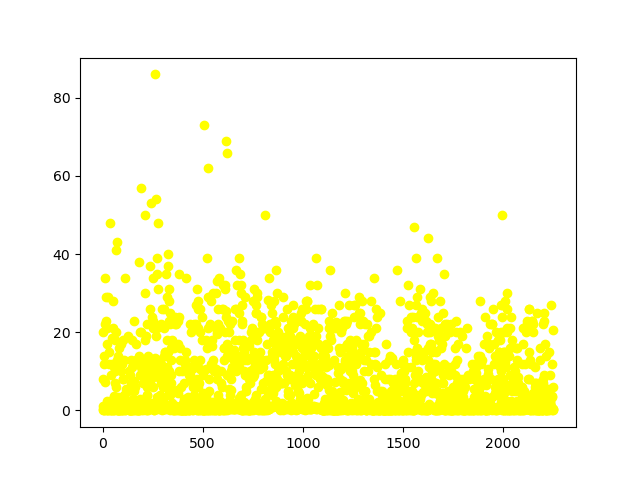
\includegraphics[width=0.5\linewidth]{Latex/sections/images/seamlesswerref.png}
    \caption{plot over the transctiption proabilites, the transcription means and the WER scores}
    \label{fig:transcript scatter plot}
\end{figure}

\section{Translation evaluation}

generate reference score with the help of comet \cite{rei-etal-2020-comet} which means that a score close to 1 is a good translation and a score close to 0 is a bad translation that is no better than random chance.
those reference scores are then also pearson correlated with the scores from the model. 
\begin{figure}[h]
    \centering
    
    \begin{subfigure}{0.4\linewidth}
        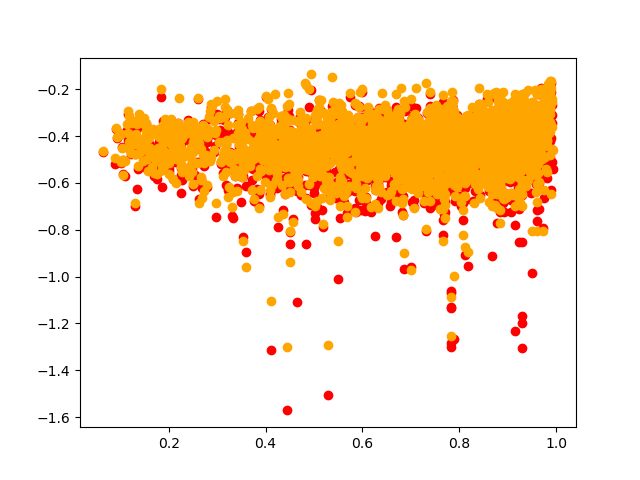
\includegraphics[width=\textwidth]{Latex/sections/images/seamlessprob.png}
    \end{subfigure}
    \begin{subfigure}{0.4\linewidth}
        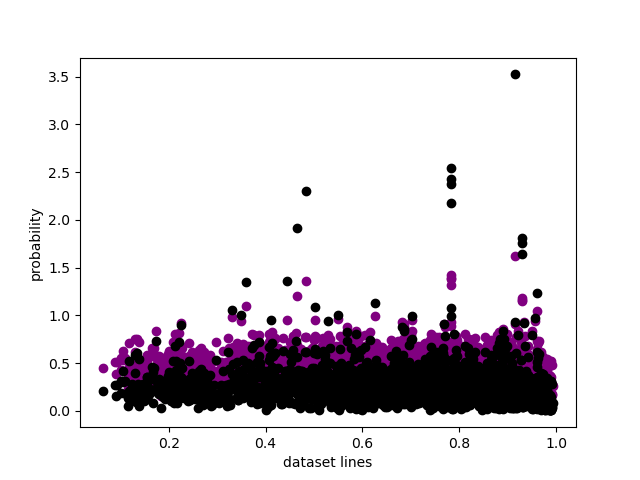
\includegraphics[width=\textwidth]{Latex/sections/images/seamlessdivanddropout.png}
    \end{subfigure}
    \begin{subfigure}{0.4\linewidth}
        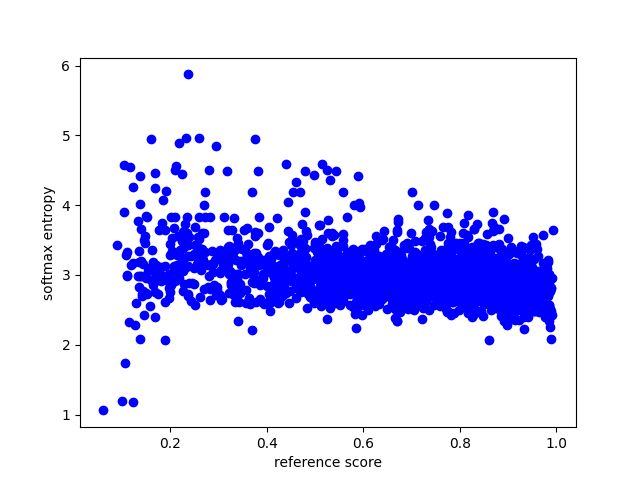
\includegraphics[width=\textwidth]{Latex/sections/images/seamlessentropy.png}
    \end{subfigure}
    
    \caption{Plot over the translation probabilities and the reference scores}
    \label{fig:translationeval scatter plot}
\end{figure}

\todo{add (scatter)plot, expand, compare results from seamless to dlm and the end to end scores add comparison with meteor}

\section{Dropout evaluation}
the dropout score is calculated by taking the mean of the dropout probabilities of the model, the variance of the dropout probabilities and a combination of both, the dropout score is then Pearson correlated with the comet scores or the word error scores in the case of the transcription. 
The correlation results are listed in \ref{results} for the translation part and \ref{transcription results} for the transcription dropout. 
%for this the dropout probabilities are calculated by running the model 30 times with the dropout layer enabled and then taking the mean and variance of the resulting probabilities. 
\todo{add text, explain results, compare them, add scatter plot}

\begin{figure}[ht]
    \centering
    \begin{subfigure}{0.4\linewidth}
    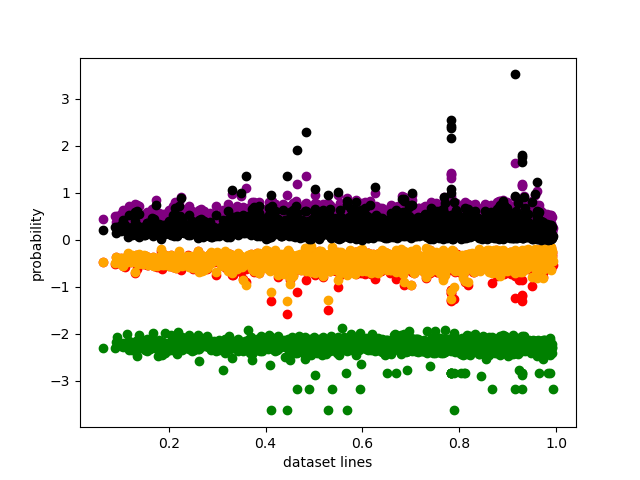
\includegraphics[width=\textwidth]{Latex/sections/images/seamlessscoresoverref.png}
    \end{subfigure}
    \begin{subfigure}{0.4\linewidth}
    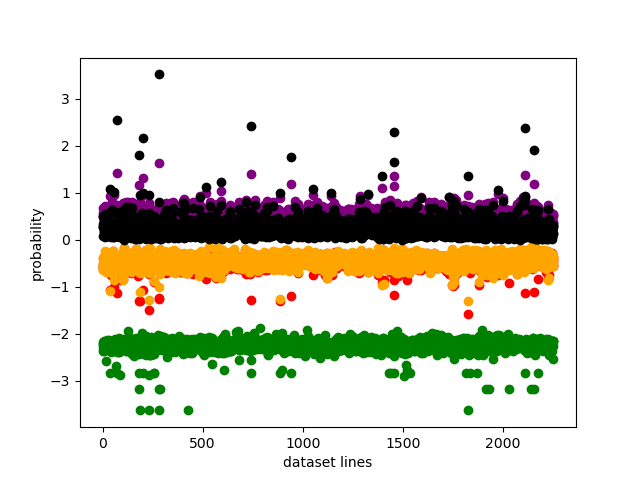
\includegraphics[width=\linewidth]{Latex/sections/images/seamlessscores.png}
    \end{subfigure}
    
    \caption{plot over the dropout translation probabilites, the variances and the references}
    \label{fig:dropout scatter plot}
\end{figure}

\section{One unified score}
since several different metrics are used in the translation part of the cascaded model it is interesting which one might be the best choice to use in a unified score, from the text translation paper \cite{fomicheva2020unsupervised} we can gather that different metrics work better for different language groups, as this thesis only tested on english to german translation no definite choice can be made without looking at other languages as well.
\todo{expand, add full judgement}

For a unified score the baselines, which are the translation and transcription probability, are multiplied. 

the resulting pearson score that can be found in \ref{results} is calculated by correlating this unified score, product of translation probability and transcription probability, with the the comet score multiplied by the by the WER mapped to be from 0 to 1 by dividing all WER scores by the worst, so highest, WER score in the dataset (alt. just setting it to 100) and subtracting it from 1. 
This is can be described mathematically as 
$$reference = cometscore*(1-\frac{WER}{max(WER)})$$
which was choosen since the transcription probability is anti-correlated to the wer and since the best score of the WER is 0 that had to be taken into account as it ruled out just flat out dividing the comet score by the WER.\\

Alternatively a unified score can be achieved by weighing the translation and transcription probabilities differently, which results in the formula $$unifiedscore_\alpha= \alpha TP_{transcript} \cdot (1-\alpha)TP_{translation}$$. 
\todo{add graph and evaluation}

\section{Pearsoncorrelation scores}
\begin{table}[ht]
  \begin{tabular}
  {l|llll}
  &  Whisper \\ \hline
  Transcription Probability& -0.33164 \\
  Transription mean & -0.60496 \\ \hline
  Dropout transcription & -0.27601 \\
  dropout variance &  0.12333\\
  dropout mean variance & - 0.087321\\
  \end{tabular}

  \caption{result from the transcription part of the cascaded model, correlatated with WER scores, with the reference and model transcript normalized}
    \label{transcription results}
\end{table}

\begin{table}[ht]
\begin{tabular}{l|llll}
    & Seamless & $\Delta$LM&  Seamless e2e\\ \hline
Translation & 0.37592 & 0.28284 & 0.656299\\ 
Softmax Entropy & -0.30604   &-0.18071 & -0.60334 \\
Standard deviation & -0.32905  & -0.25363& -0.67148 \\ \hline

Dropout translation & 0.150755& 0.282556& 0.14194\\

Dropout Variance &-0.106986 & -0.16285& 0.13080\\
Dropout combo & -0.163593& 0.17962061& -0.20624\\
\hline
unified score   & -0.32965 &  & - 
%{transcription'pearsonr': -0.3258220972065334} transcription mean {'pearsonr': -0.27601804379827566}

%dlm probabilitycorrelation {'pearsonr': 0.2828435783527934} softmaxcorrelation {'pearsonr': -0.08377165154268117 or  -0.083771} std correlation {'pearsonr': -0.2536297836740317} dp prob corr {'pearsonr': 0.2825563734152303} dp var corr {'pearsonr': -0.1628538934576183} dpcombo {'pearsonr': 0.17962061402392054}
%seamless dropout {'pearsonr': 0.08839374531318331} {'pearsonr': -0.0962085313546643}  
\end{tabular}

\caption{Correlation scores for the separate models and calculated quality scores}
\label{results}
\end{table}

other interesting values: the pearson correlation of the entropies in dropout shows a significant prediction value with a correlation of the mean of -0.23241 and a correlation of -0.17032 of the variance of the entropies on seamless.